% Use only LaTeX2e, calling the article.cls class and 12-point type.

\documentclass[11pt]{article}
\usepackage[round,semicolon]{natbib}
\usepackage[margin=1.4in]{geometry}
\usepackage{kpfonts}

\usepackage{seqsplit}
\usepackage{placeins}

\usepackage{newfloat}
\usepackage[labelfont=bf]{caption}
\usepackage{nameref}
\usepackage{rotating}
\usepackage{color}
\usepackage{float}

\setcounter{topnumber}{8}
\setcounter{bottomnumber}{8}
\setcounter{totalnumber}{8}

\usepackage{newfloat}
\DeclareFloatingEnvironment[name={Figure}]{suppfigure}
\renewcommand{\thesuppfigure}{S\arabic{suppfigure}}

\definecolor{darkblue}{rgb}{0, 0.0, 0.6}

\usepackage{hyperref}
\hypersetup{colorlinks,citecolor=blue,linkcolor=darkblue,urlcolor=blue}

\usepackage{seqsplit}

\usepackage{array}
\newcolumntype{R}[1]{>{\raggedright\arraybackslash}p{#1}}
\newcolumntype{C}[1]{>{\centering\let\newline\\\arraybackslash\hspace{0pt}}m{#1}}

\newcommand{\comment}[1]{{\color{red}[\textsl{#1}]}}

\usepackage{setspace}

\renewcommand{\topfraction}{1}
\renewcommand{\bottomfraction}{1}
\renewcommand{\textfraction}{0}
\renewcommand{\floatpagefraction}{1}

%\renewcommand{\abstractname}{\large SUMMARY}


\title{Quantifying the ease of viral escape from broad and narrow antibodies to influenza hemagglutinin} 

\author
{Michael B. Doud$^{1,2,3,\dagger}$, Juhye M. Lee$^{1,2,3,\dagger}$, and Jesse D. Bloom$^{1,2,*}$\\
\\
\scriptsize{$^1$Basic Sciences and Computational Biology Program, Fred Hutchinson Cancer Research Center}\\
\scriptsize{$^2$Department of Genome Sciences and $^3$Medical Scientist Training Program, University of Washington} \\
\scriptsize{Seattle, WA, USA} \\
\scriptsize{$^{\dagger}$These authors contributed equally} \\
\scriptsize{$^*$Correspondence: \href{jbloom@fredhutch.org}{jbloom@fredhutch.org}}
}

\date{}


\begin{document}

\maketitle
\onehalfspacing

\begin{abstract}
Influenza virus can completely escape most antibodies with single mutations.
However, rare antibodies broadly neutralize many viral strains.
It is unclear how easily influenza virus might escape such broad antibodies if they became widespread due to therapeutic use or vaccination.
Here we map all single amino-acid mutations that increase resistance to broad antibodies targeting hemagglutinin.
Crucially, our approach not only identifies antigenic mutations but also quantifies their effect sizes.
All antibodies select mutations, but the effect sizes vary widely. 
The virus can escape a broad antibody targeting hemagglutinin's receptor-binding pocket the same way it escapes narrow strain-specific antibodies: via single mutations with huge effects.   
In contrast, broad antibodies targeting hemagglutinin's stalk only select mutations with small antigenic effects. 
Therefore, antibody breadth is not necessarily an indicator of the difficulty of viral escape.
Broad antibodies targeting hemagglutinin's stalk are quantifiably harder to escape than antibodies targeting hemagglutinin's head or receptor-binding pocket.
\end{abstract}

\section*{INTRODUCTION}
Nearly all viruses show some antigenic variation.
However, the extent of this variation ranges widely.
For instance, although both measles virus~\citep{birrer1981antigenic,ter1981antigenic} and polio virus~\citep{crainic1983natural,diamond1985antigenic,drexler2014robustness} exhibit antigenic variation, the magnitude of this variation is small. 
Therefore, immunity elicited by infection or vaccination provides life-long protection against both these viruses~\citep{?}.
In contrast, some other viruses exhibit much more extensive antigenic variation.
An example is human influenza virus.
Infection with influenza virus provides life-long immunity to the infecting strain~\citep{?}.
But influenza virus undergoes such rapid antigenic evolution that the effectiveness of this immunity to antigenically drifted viral strains is almost completely eroded within a few years~\citep{?}. 

Many explanations have been suggested for the differences in extent of antigenic variation among viruses, including epidemiological factors, the breadth of the immune response, and the virus's inherent evolutionary capacity to escape immunodominant antibody specificities~\citep{lipsitch2007patterns,cobey2014pathogen,fulton2015mutational}.
Here we will focus on the last of these explanations, as it provides the underlying rationale for recent efforts to develop a ``universal'' influenza vaccine that protects against a wide range of viral strains.

According to this inherent evolutionary capacity explanation, human influenza virus undergoes rapid antigenic drift because most neutralizing antibodies target epitopes on the viral hemagglutinin protein that are highly tolerant of mutational change.
This explanation is supported by classic experiments showing that it is easy to select viral mutants that completely escape most anti-hemagglutinin antibodies~\citep{}, as well as by the observation that single mutations that cause large changes in antigenicity arise frequently during the natural evolution of human influenza virus at the global scale~\cite{?} and even within individual humans with long-term infections~\cite{?}.
A corollary of this explanation is that the virus's capacity for antigenic drift would be greatly reduced if most antibodies instead targeted epitopes 

This corollary has become of more than academic interest with the discovery of broadly neutralizing antibodies.

Of course, it remains unclear if these epitopes are more conserved because they are inherent intolerant or just aren't under pressure.
For instance, non-human influenza doesn't undergo much antigenic drift.
Knowing is important because success of a vaccine would put them under pressure.

Broadly neutralizing antibodies against influenza virus are of great interest... \cite{corti2017tackling}. 

% blurbs about the specific antibodies we use here:
C179 isolation and escape mutant selection \cite{okuno1993common}.
C179 structure with 1957 H2, binding data to many strains, and citations to older studies demonstrating C179 cross-neutralization to H1, H2, H5, H6, and H9:  \cite{dreyfus2013structure}.
FI6v3 was isolated... \cite{corti2011neutralizing}.
S139/1 isolation and selection of escape mutants from Aichi H3, Adachi H2, and WSN H1: \cite{yoshida2009cross}.
S139/1 structure with Victoria75 H3 and binding/neutralization data: \cite{lee2012heterosubtypic}.

Recently we have described new technologies... \cite{doud2017complete, dingens2017comprehensive}.


\section*{RESULTS}

\subsection*{A method to quantify the ease of escape.}
\comment{Jesse writes a draft of this section.}
\begin{figure}
\centerline{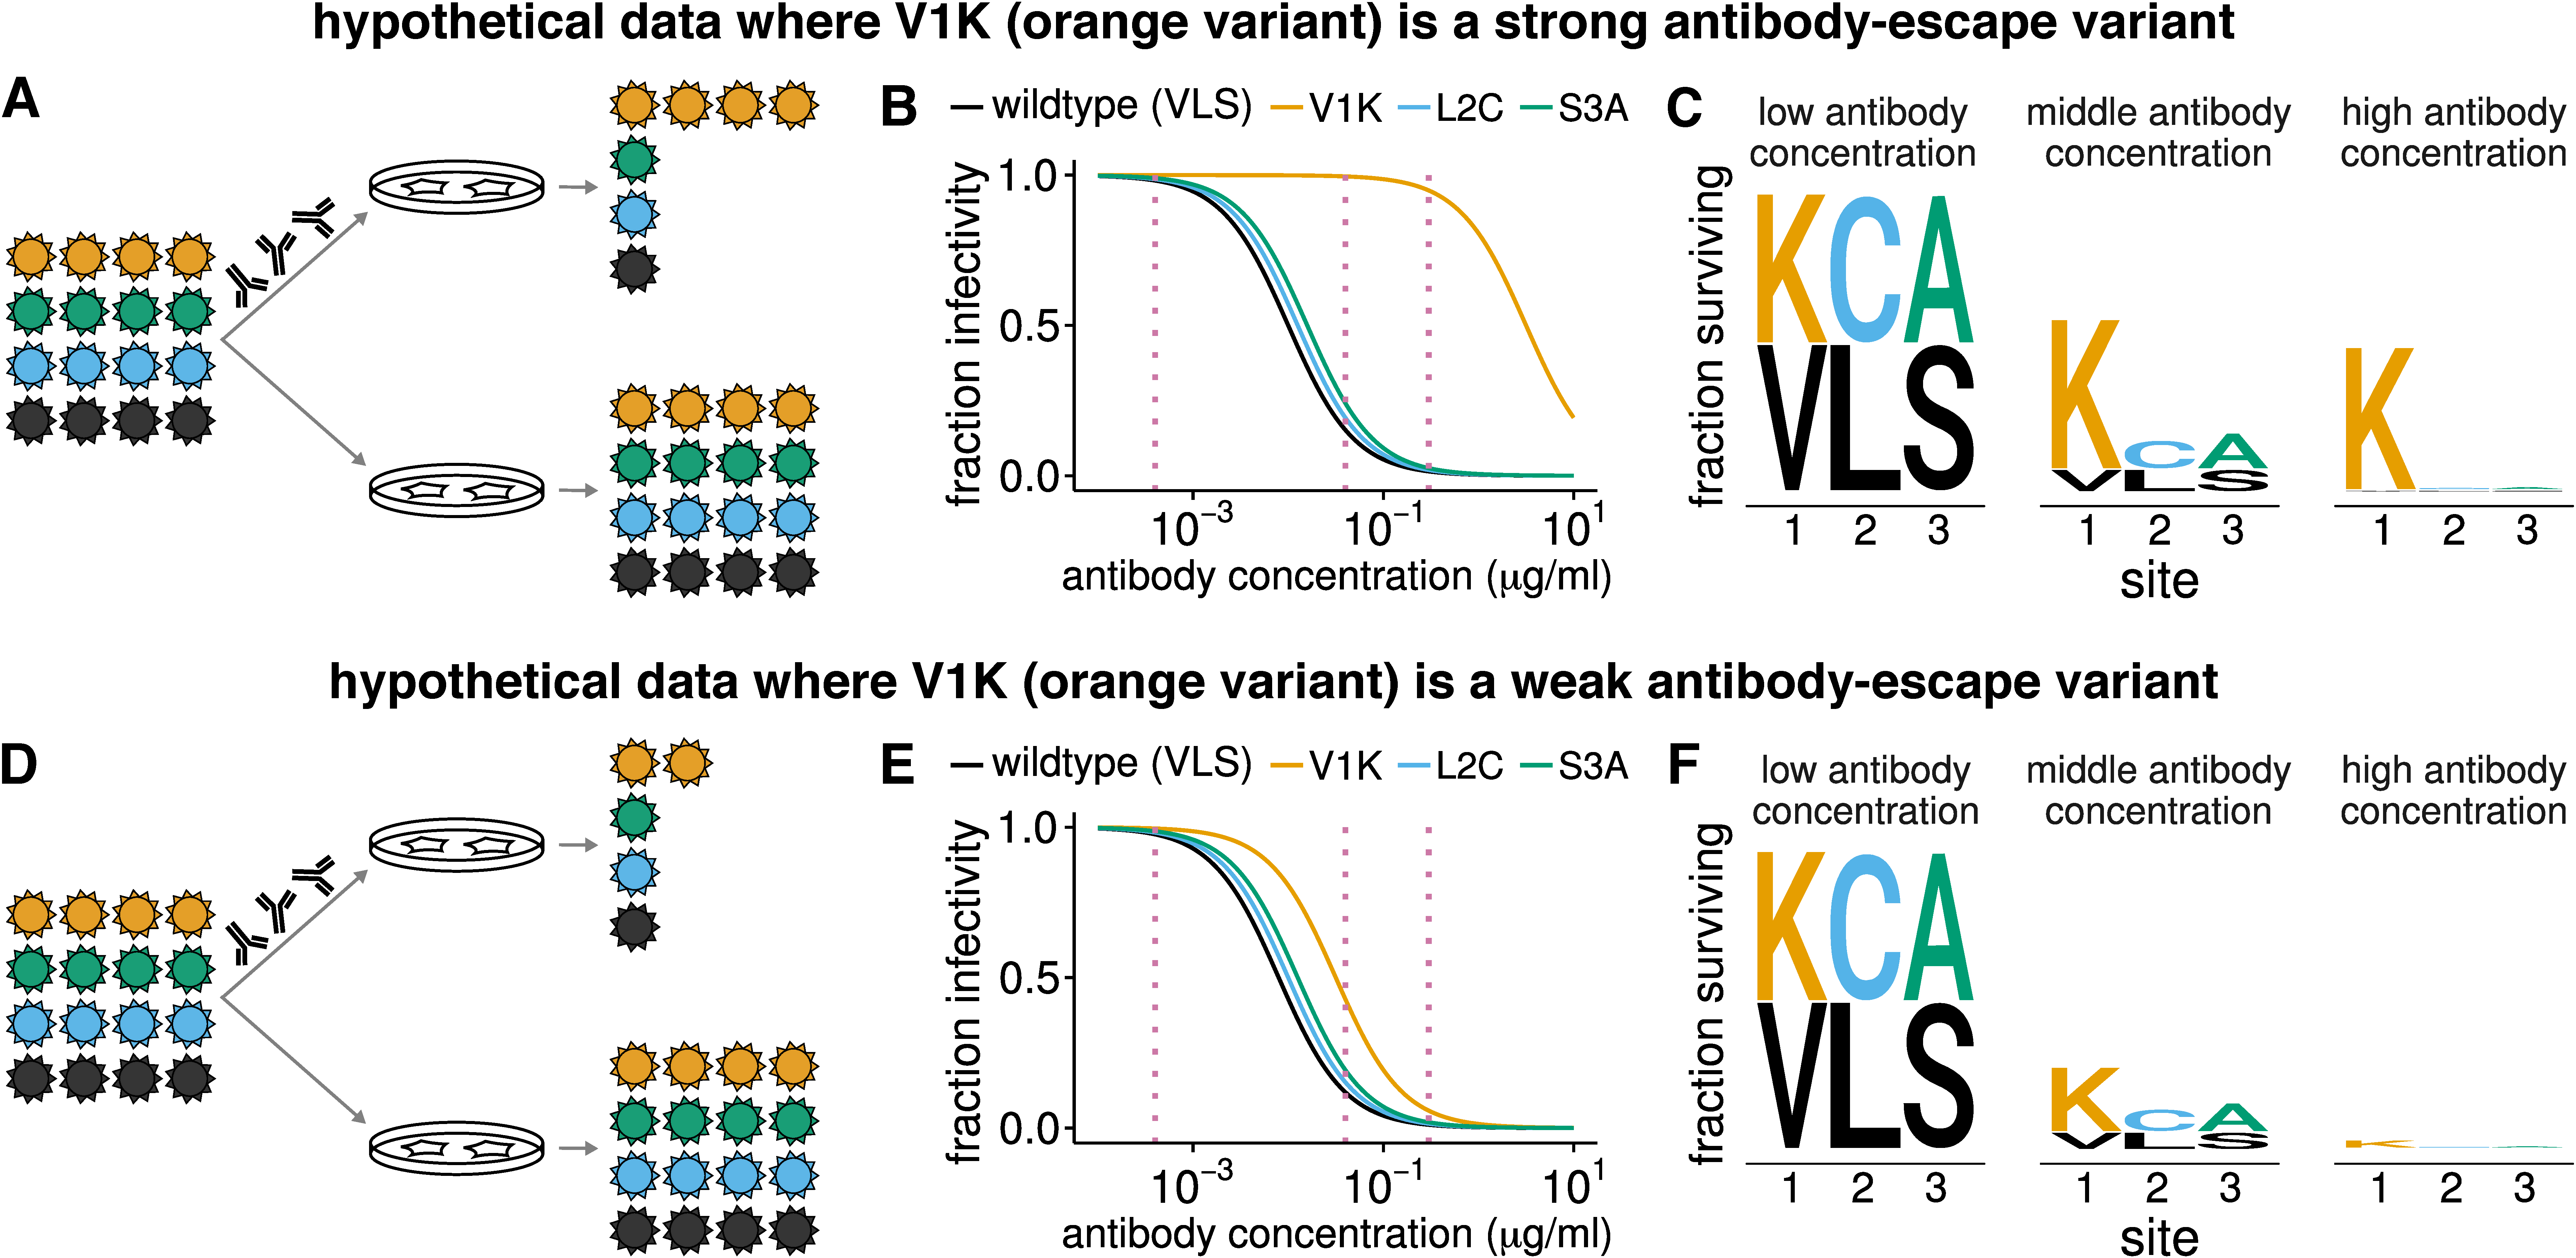
\includegraphics[width=\textwidth]{figs/fracsurvive_example/fracsurvive_fig.pdf}}
\caption{\label{fig:fracsurvive_example}
CAPTION
\comment{One additional change to this figure: can you increase the spacing between panels, especially the top and bottom set of panels but also a bit between the ones on the same horizontal level. Right now it is too crowded.}
}
\end{figure}

\subsection*{Broad and narrow antibodies that neutralize influenza virus hemagglutinin}
\comment{Juhye writes a draft of this section.}
\begin{figure}
\centerline{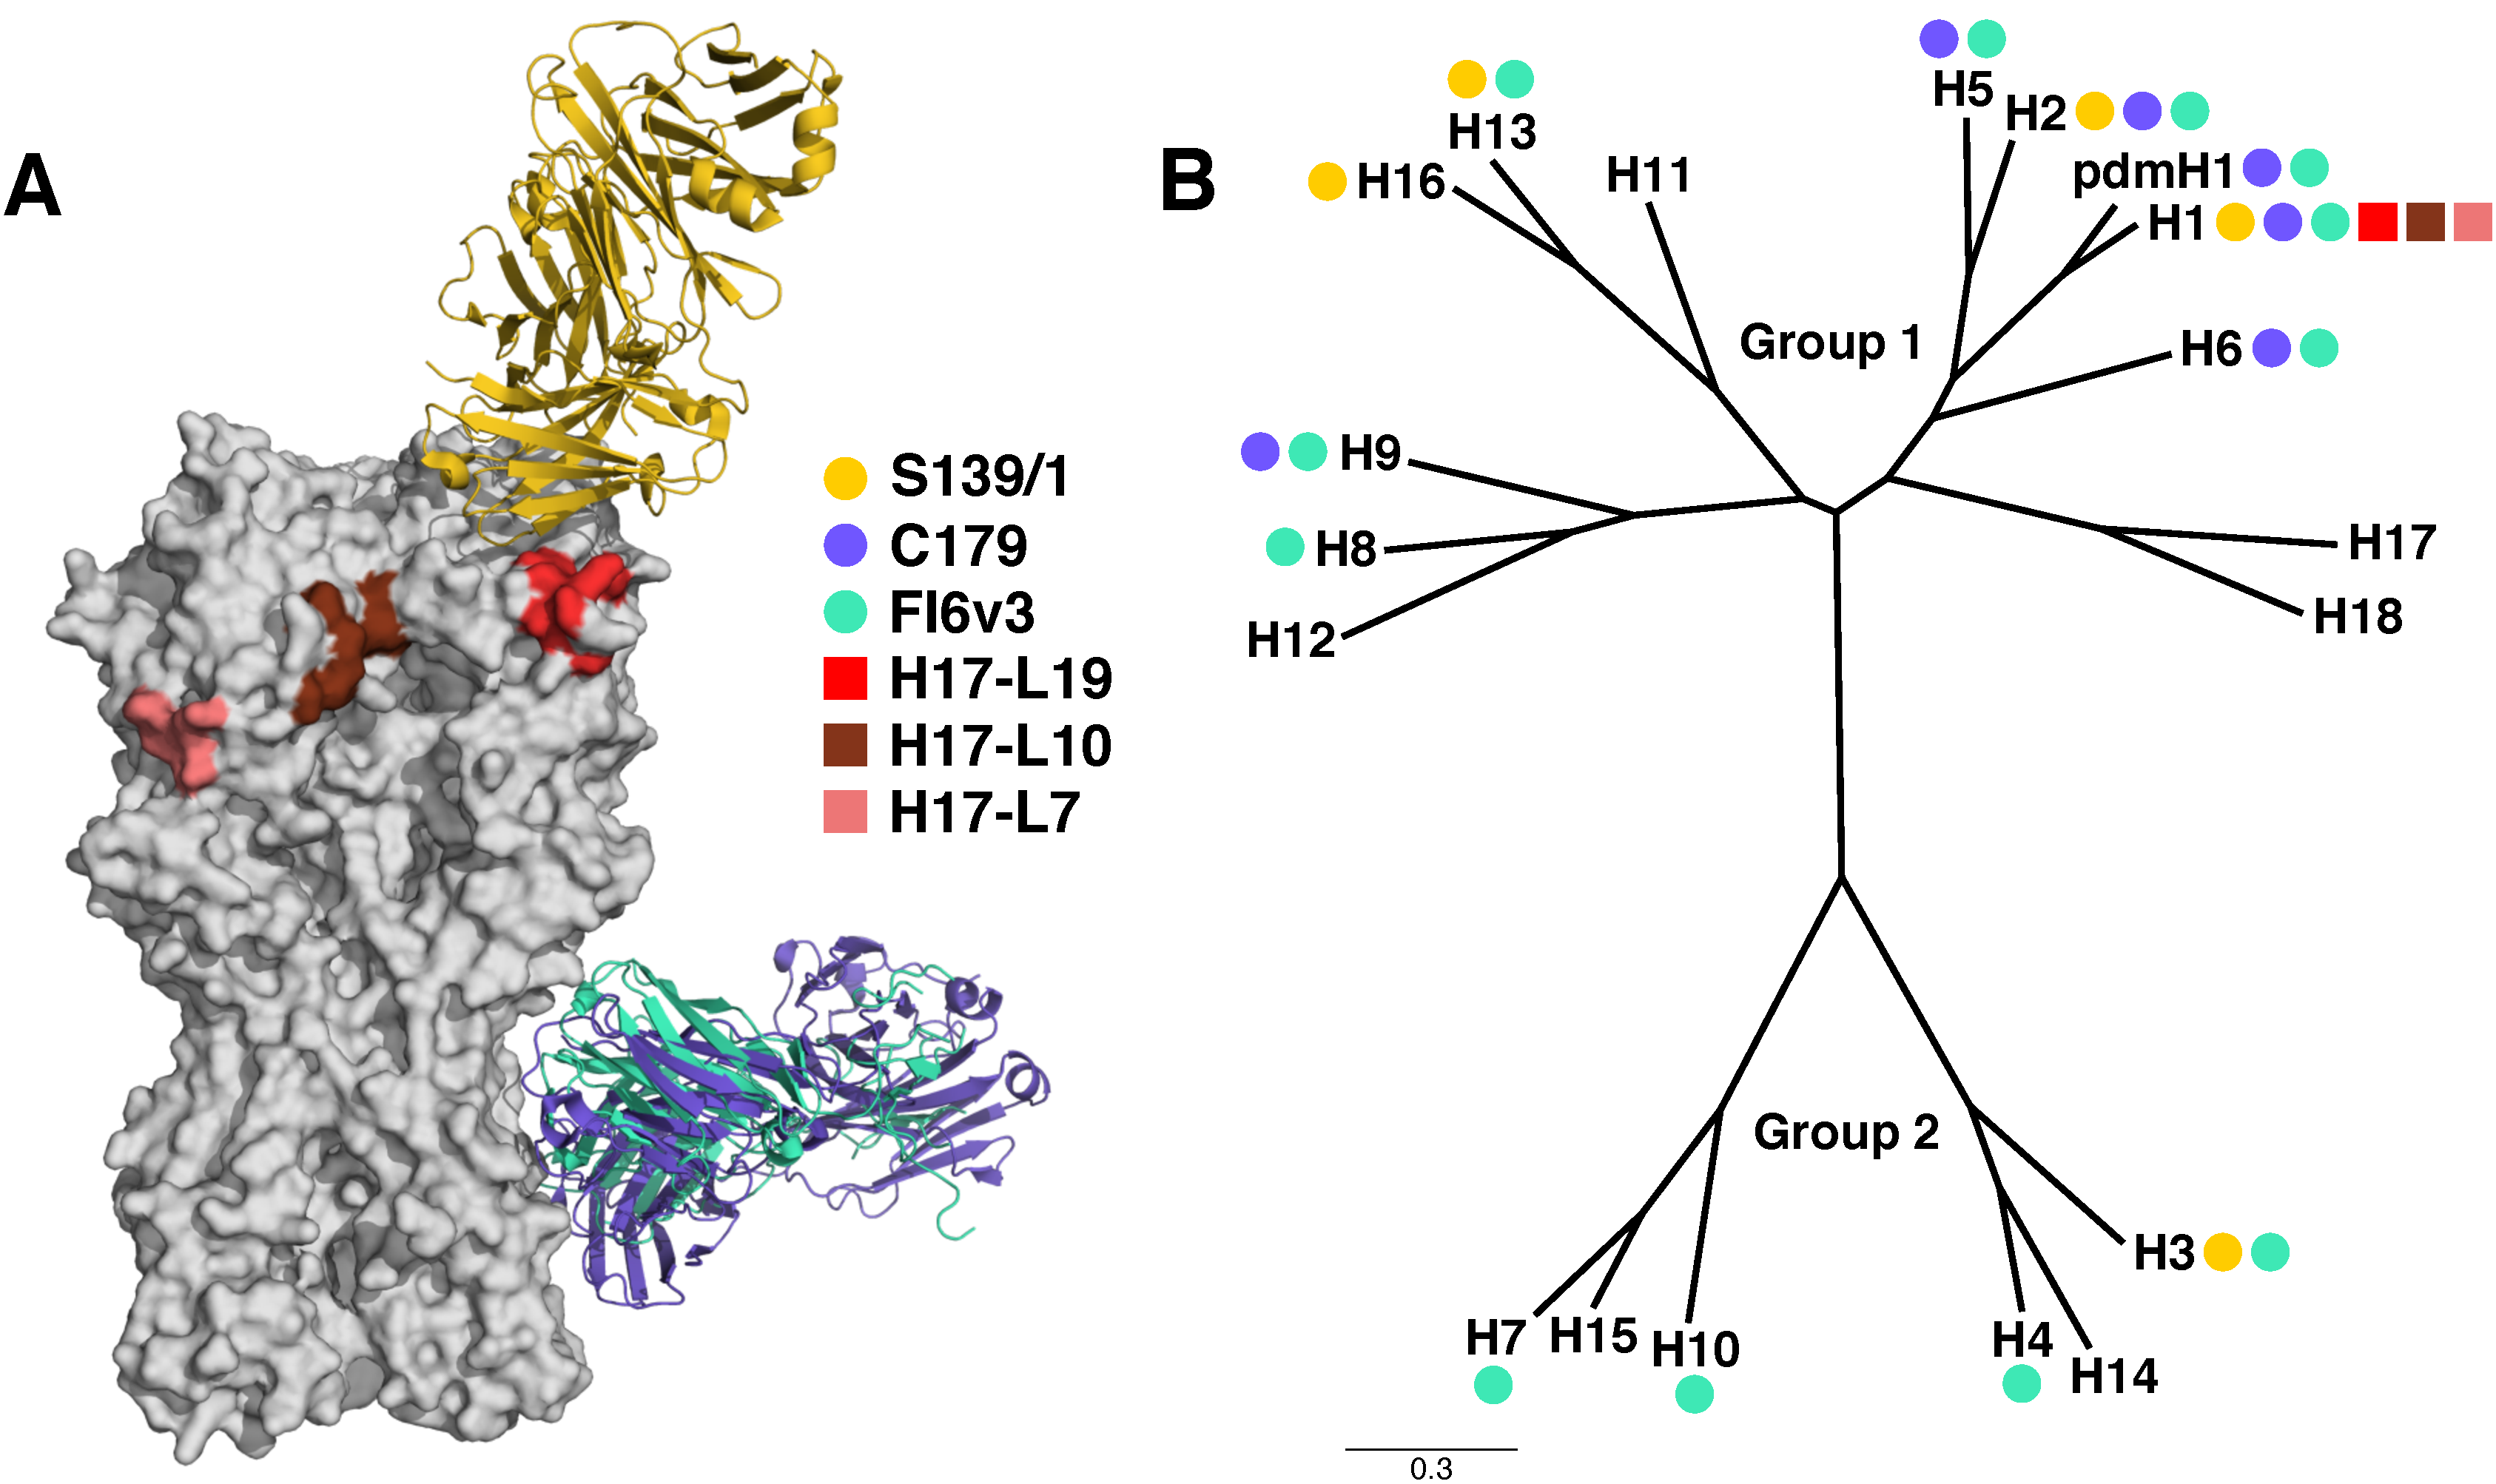
\includegraphics[width=\textwidth]{figs/antibody_summary_fig/Ab_summary.pdf}}
\caption{\label{fig:antibody_summary}
CAPTION
}
\end{figure}


\begin{figure}
\centerline{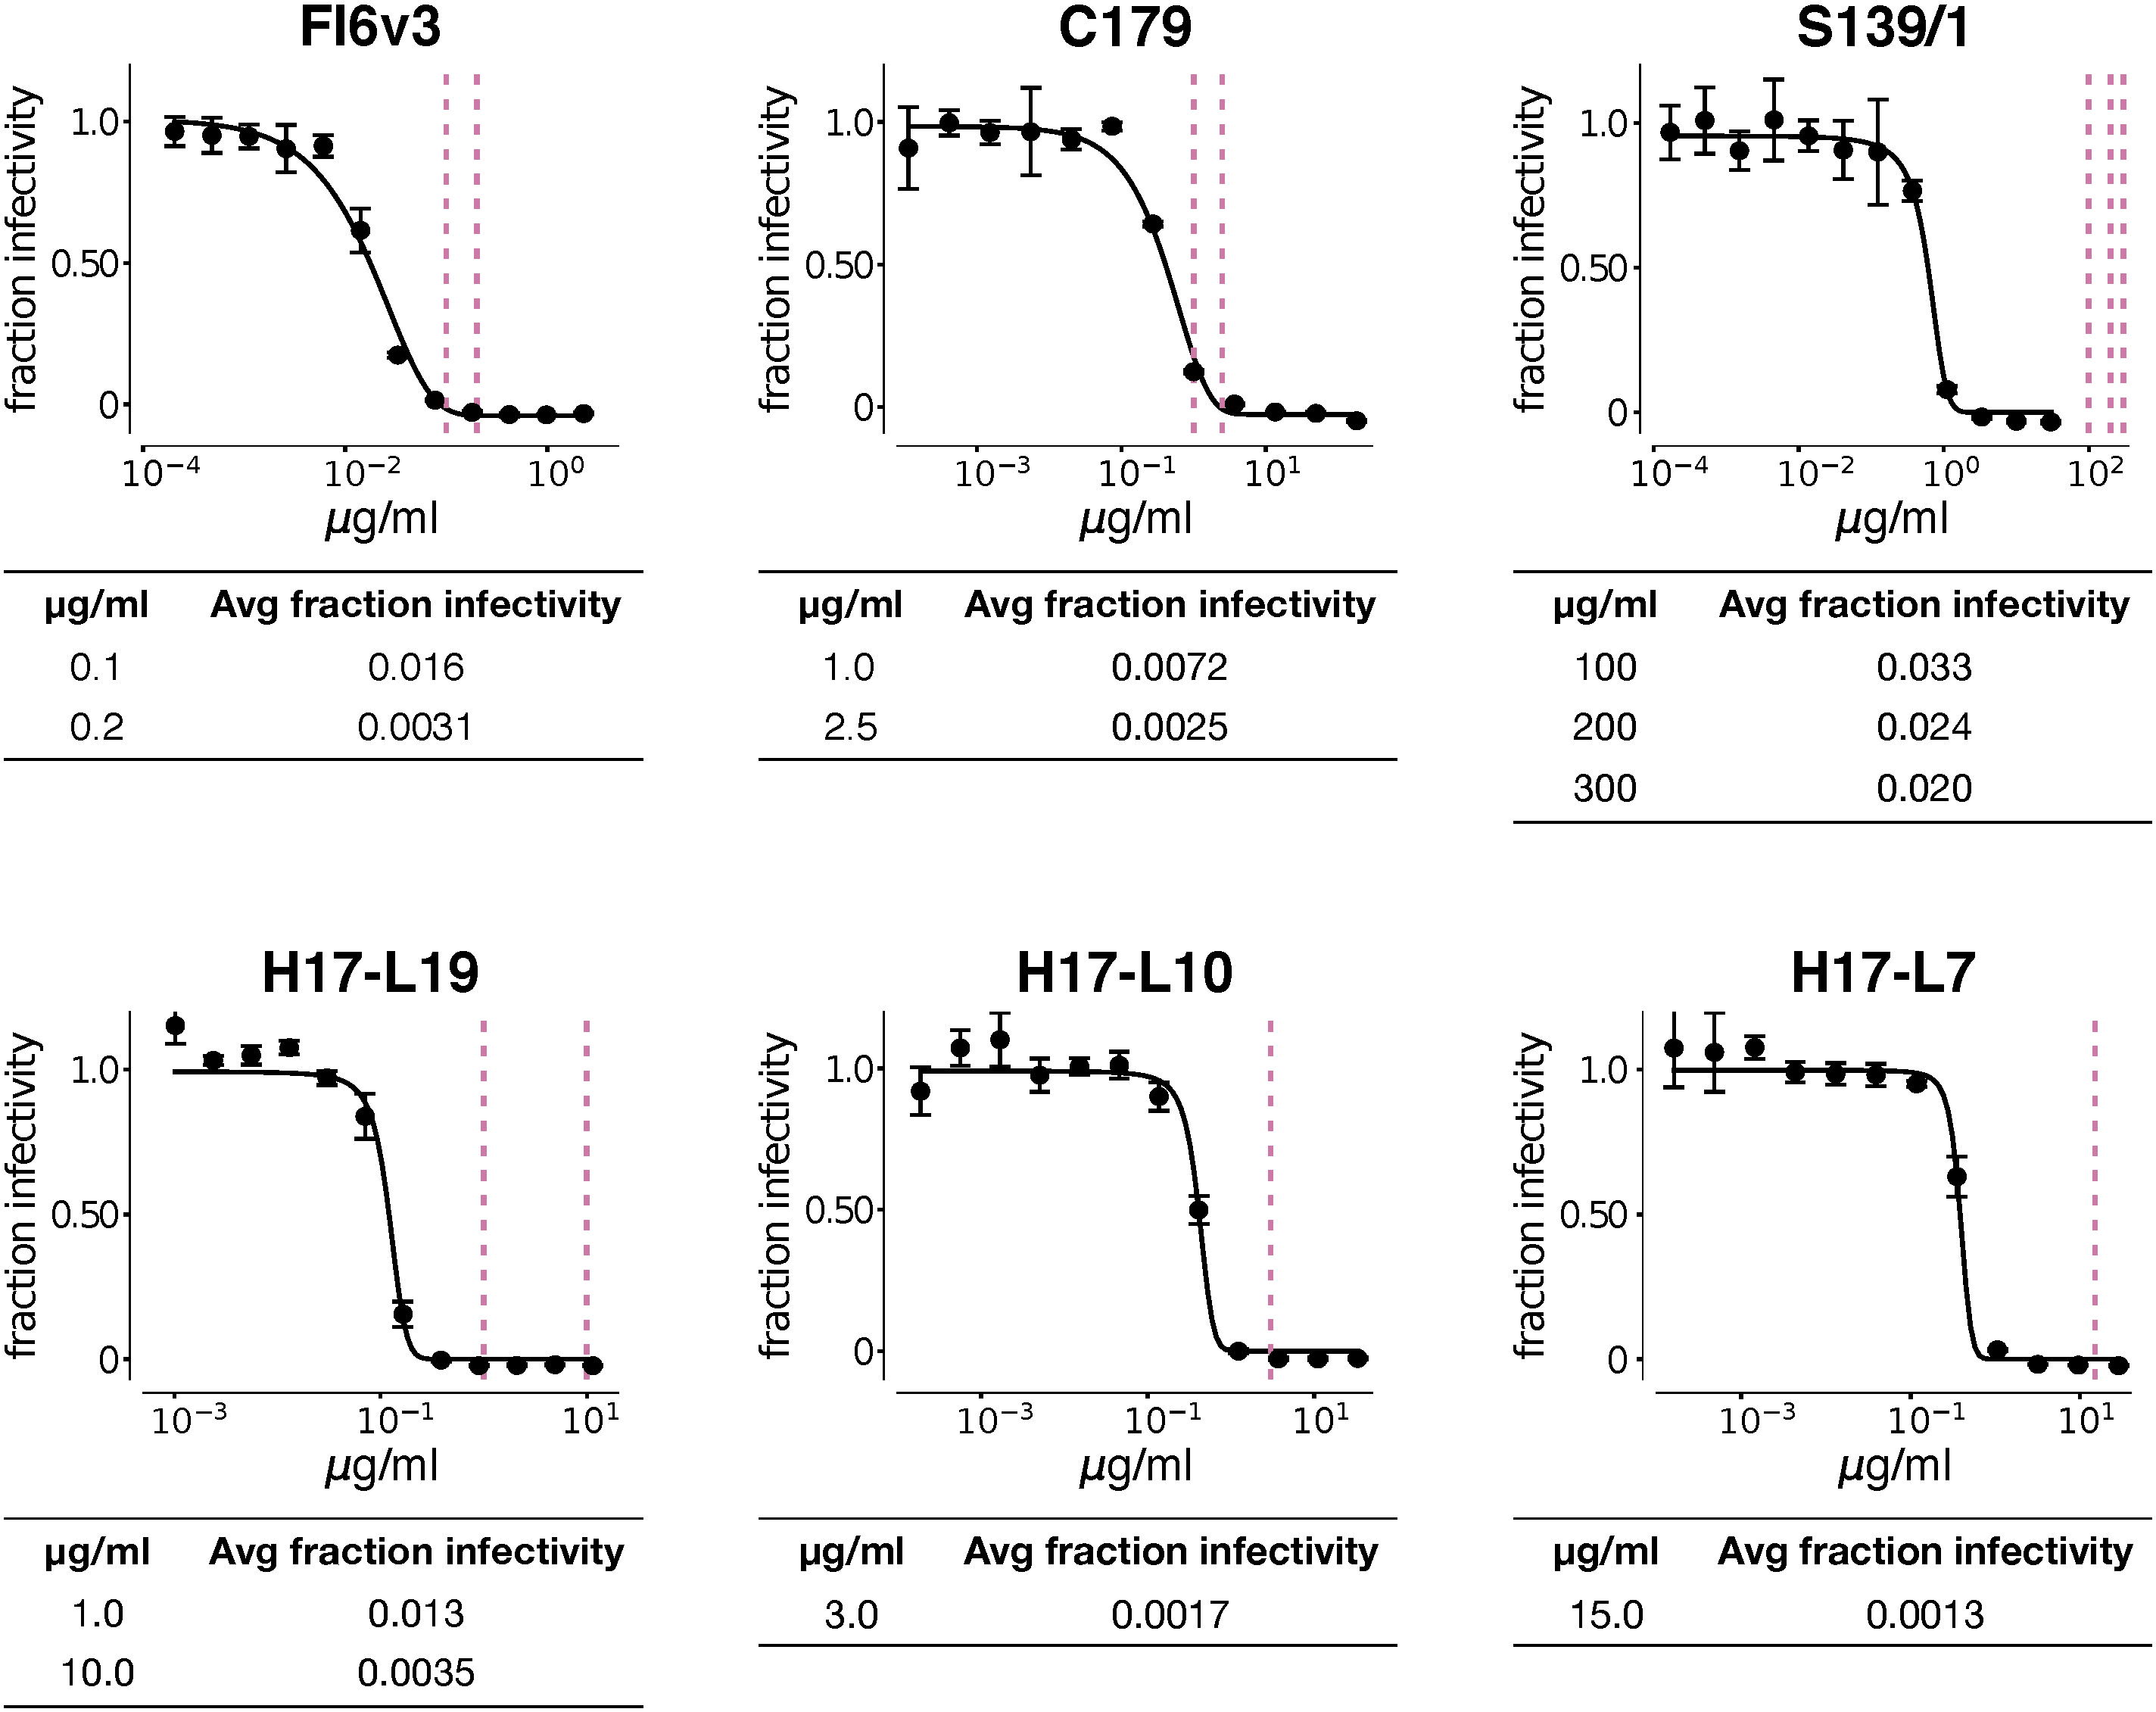
\includegraphics[width=0.8\textwidth]{figs/neutralization_curves/WT_neutralization_curves.pdf}}
\caption{\label{fig:neutcurves}
CAPTION
\comment{Can you modify this plot to bring the formatting more in line with Figure~\ref{fig:fracsurvive_example}. 
This includes:
(1) Make the y-axis \emph{fraction infectivity}.
(2) Make the vertical lines dotted and of the same color as in Figure~\ref{fig:fracsurvive_example}, which is the last color in the \emph{cbbPalette} defined here \url{https://github.com/jbloomlab/HA_antibody_ease_of_escape/blob/master/paper/figs/fracsurvive_example/fracsurvive_example.ipynb}. 
(3) Get rid of the minor tick marks that show up on two of the four plots.
(4) Add H17-L10 and H17-L9, and make the plot three antibodies per line.
(5) Get rid of the concentration of S139/1 that we are not using.
(6) Also, I think it would look better if for each plot the antibody name was just a title above the plot in large letters. The x-axis then can then just ``antibody concentration ($\mu$g/ml)''. Also, I don't think you need the number labels for the concentrations on either the plot or in the table. If your table has the concentration and fraction infectivity, it is obvious which line goes with which concentration just by seeing how they are arranged horizontally.
(7) Increase the font size in the table (you'll have more space to do this after you get rid of the numbers).
}
}
\end{figure}

\subsection*{Ease of escape from each antibody}
This would show the medianavgfracsurvive plot.

\begin{figure}
\centerline{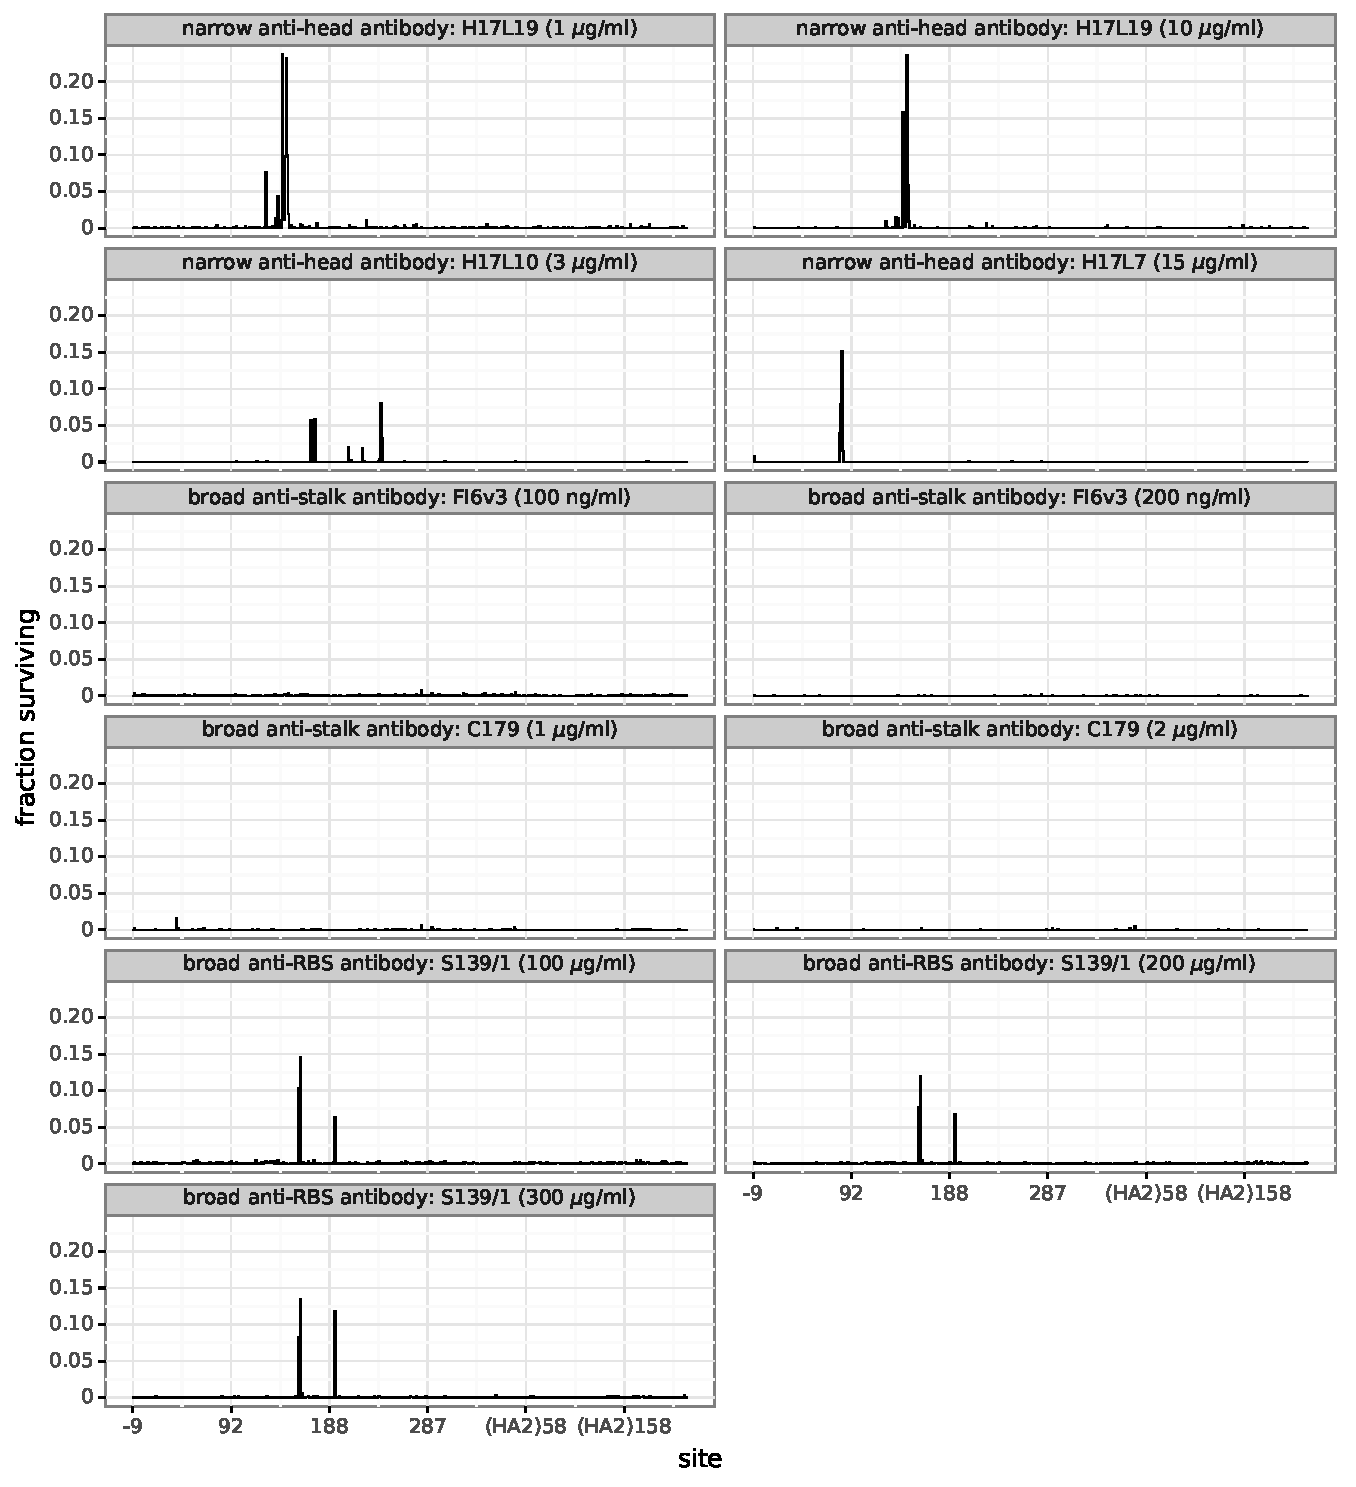
\includegraphics[width=\textwidth]{figs/avgfracsurvive.pdf}}
\caption{
\label{fig:avgfracsurvive}
CAPTION
Figure~\ref{suppfig:maxfracsurvive} shows the fraction surviving for the single most strongly selected amino-acid mutation at each site.
}
\end{figure}

\subsection*{For all antibodies, the selected sites of escape occur in the antibody binding footprints}

\section*{DISCUSSION}
Some discussion

\clearpage

\section*{METHODS}
\subsection*{Antibodies}
FI6v3 was expressed and purified by the Fred Hutchinson Cancer Research Center protein expression core \comment{i think?}.
C179 was purchased from Takara Bio Inc (Catalog \# M145).
S139/1 heavy and light chain variable sequences were obtained from PDB ID 4GMS~\cite{lee2012heterosubtypic} and expressed and purified by the Fred Hutchinson Cancer Research Center protein expression core.

\subsection*{Mutant virus selections with antibody}
Library selections, deep sequencing, and computation of mutation differential selection were performed as previously described~\cite{doud2017complete}. Briefly, ...

\subsection*{Computation of the fraction $\phi_{r,a}$ of each mutation that escapes antibody neutralization}
\comment{depending on how much of paper focus is on this new metric, some of this rationale might be better placed in the results section}

Mutation differential selection values $s_{r,a}$ reflect the enrichment of a mutation in an antibody-selected sample relative to a mock-selected control. 
The extent of these mutation enrichments are dependent on the stringency of the neutralization: as the concentration of an antibody used to neutralize the mutant virus library is increased, a larger proportion of the virus library is neutralized, and escape mutants become more enriched in the antibody-selected sample relative to the control sample~\cite{doud2017complete}.
Consequently, due to differences in the concentrations and potencies of various antibodies used in mutational antigenic profiling, quantitative comparisons of the effects of mutations on neutralization escape between various antibodies is confounded by differences in neutralization stringency across experiments.

We defined a new metric that accounts for the neutralization stringency of each experiment so that quantitative comparisons can be made between experiments with varying neutralization stringencies.
This new measure, $\phi_{r,a}$, is roughly analogous to the fraction of mutant viruses carrying mutation $a$ at site $r$ that escape neutralization by a given antibody.
The computation of $\phi_{r,a}$ incorporates information about the stringency of neutralization. 
We define this as  $\gamma$ = (100 - \% neutralization)/100), the fraction of library remaining infectious after antibody neutralization measured by qRT-PCR for each antibody-selection experiment as previously described~\cite{doud2017complete}.

Define $\hat{n}_{r,a}^{sel}$ and $\hat{n}_{r,a}^{mock}$ as the number of error-corrected counts of amino-acid mutant $a$ at site $r$ as defined in~\cite{doud2017complete}, and $N_r^{sel}$ and $N_r^{mock}$ be the total counts at site $r$, as specified for either an antibody selection or matched mock condition.
Let $P$ be a pseudocount (default to 5 in these analyses) added to amino-acid counts, and let $f_{r}^{sel}$ and $f_{r}^{mock}$ be relative depths of the selected and mock samples at site $r$ for the purposes of scaling the pseudocount by relative read depth as previously described~\cite{doud2017complete}.

Define the pseudocount-adjusted frequency $\rho$ of mutant $a$ at site $r$ in selected and mock samples to be:
$$\rho_{r,a}^{sel} = \frac{n_{r,a}^{sel}+f_r^{sel}\times P}{N_r^{sel}+f_r^{sel}\times  P}$$
$$\rho_{r,a}^{mock} = \frac{n_{r,a}^{mock}+f_r^{mock}\times P}{N_r^{mock}+f_r^{mock}\times  P}$$

We define $\phi_{r,a}$ as the net `fraction' of mutant $a$ at site $r$ escaping neutralization (above the average escape fraction $\gamma$), and compute this as:
$$\phi_{r,a} = \frac{\gamma \times \rho_{r,a}^{sel}}{\rho_{r,a}^{mock}} - \gamma$$

By this definition, mutations with no effect on antibody escape will have $\phi_{r,a} =0$, and mutations completely escaping antibody will have $\phi_{r,a} \approx 1$.
Care should be taken in interpreting the absolute values of $\phi$, however, since the choice of pseudocount affects the range of $\phi$ values (but not, importantly, the relationships of $\phi$ distributions across antibodies).
We have found that a value of $P=5$ pseudocounts results in $\phi$ values that are roughly bounded from 0 to 1, and consistently use $P=5$ all analyses.

\subsection*{Data availability and source code}
Deep sequencing data has been deposited at the Sequence Read Archive under BioSample accession (\comment{should probably deposit all the new data into the existing biosample SAMN05789126 (Sample name: WSN/1933 HA mutant libraries selected by monoclonal antibodies), which is under bioproject PRJNA309339}).




\clearpage

\small
\subsection*{ACKNOWLEDGMENTS}
This work was supported by grants R01GM102198 and R01AI127893 from the NIGMS and NIAID of the NIH.
MBD was supported in part by training grant T32AI083203 from the NIAID of the NIH.
JML was supported in part by \comment{CIDID grant}.
The research of JDB is supported in part by a Faculty Scholar Grant from the Howard Hughes Medical Institute and the Simons Foundation.

\bibliographystyle{mbe}
\bibliography{references.bib}

\clearpage
\normalsize

\section*{Supplementary Material}
\FloatBarrier

\begin{suppfigure}
\centerline{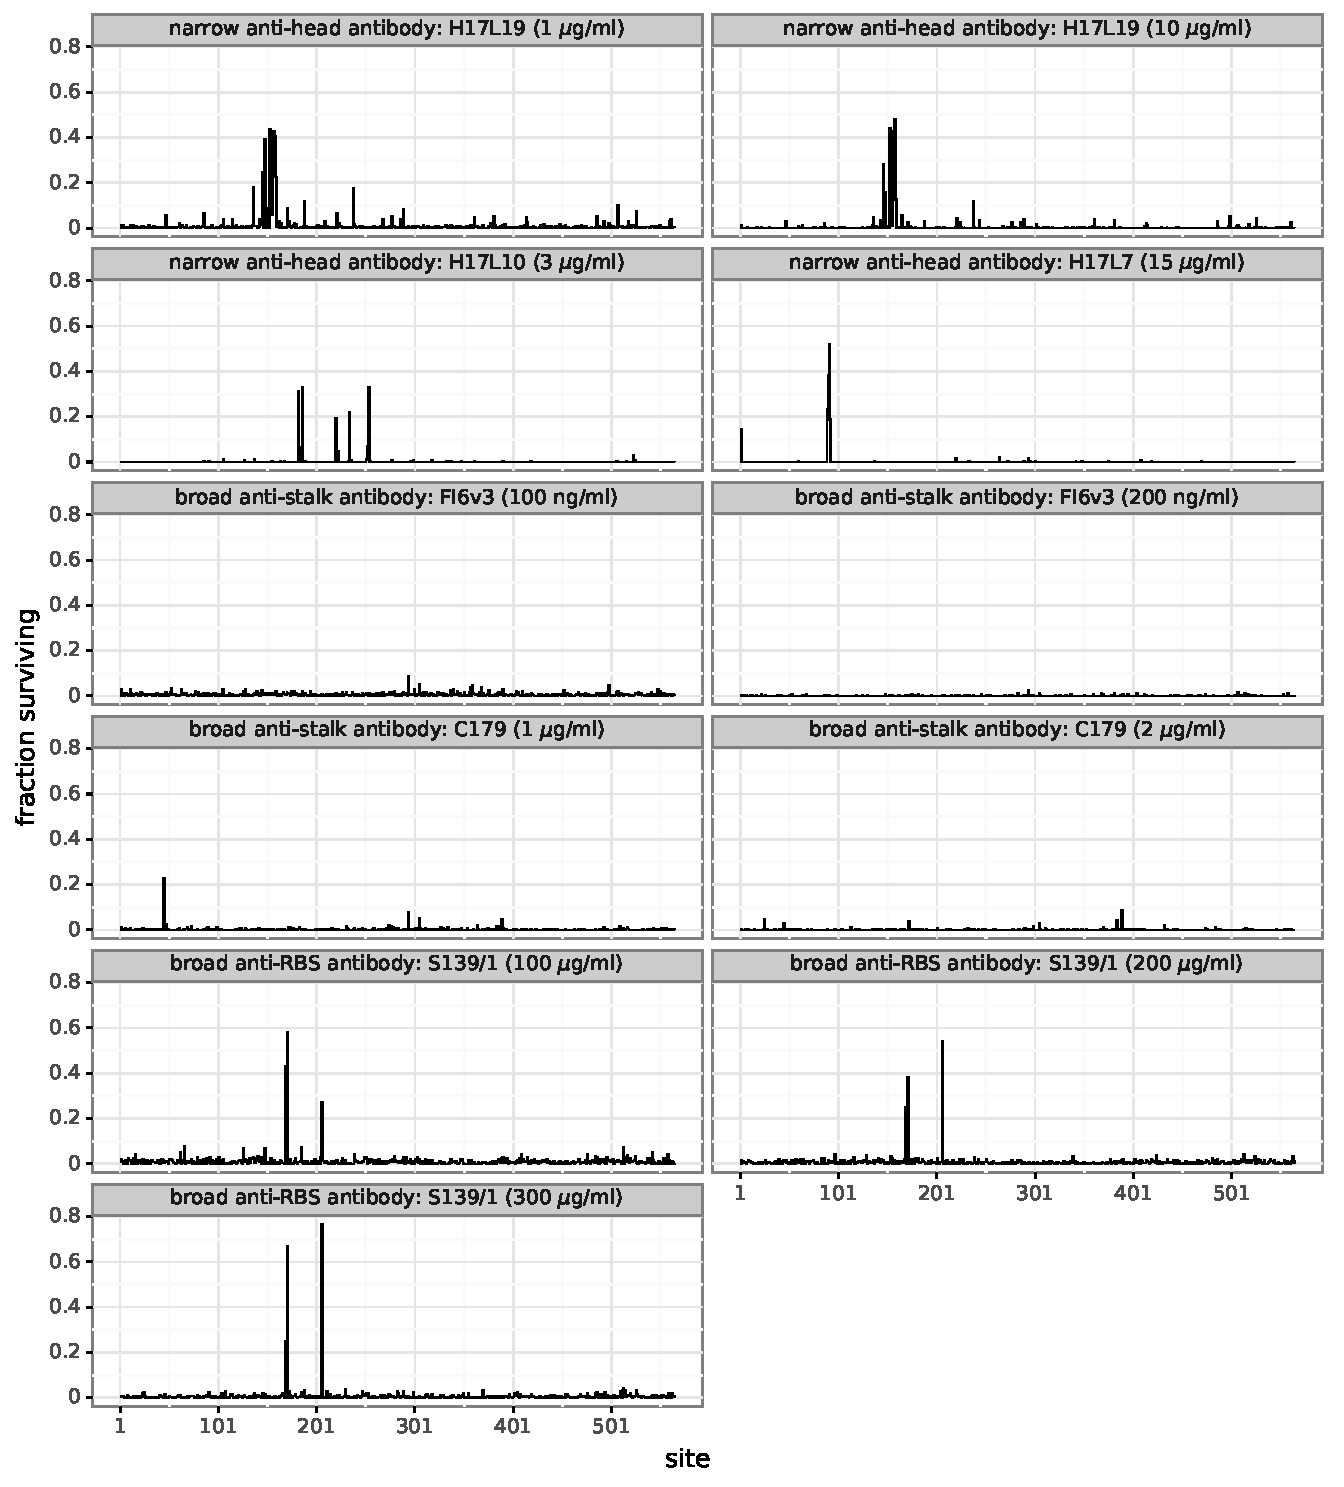
\includegraphics[width=\textwidth]{figs/maxfracsurvive.pdf}}
\caption{\label{suppfig:maxfracsurvive}
CAPTION}
\end{suppfigure}

\begin{suppfigure}
\centerline{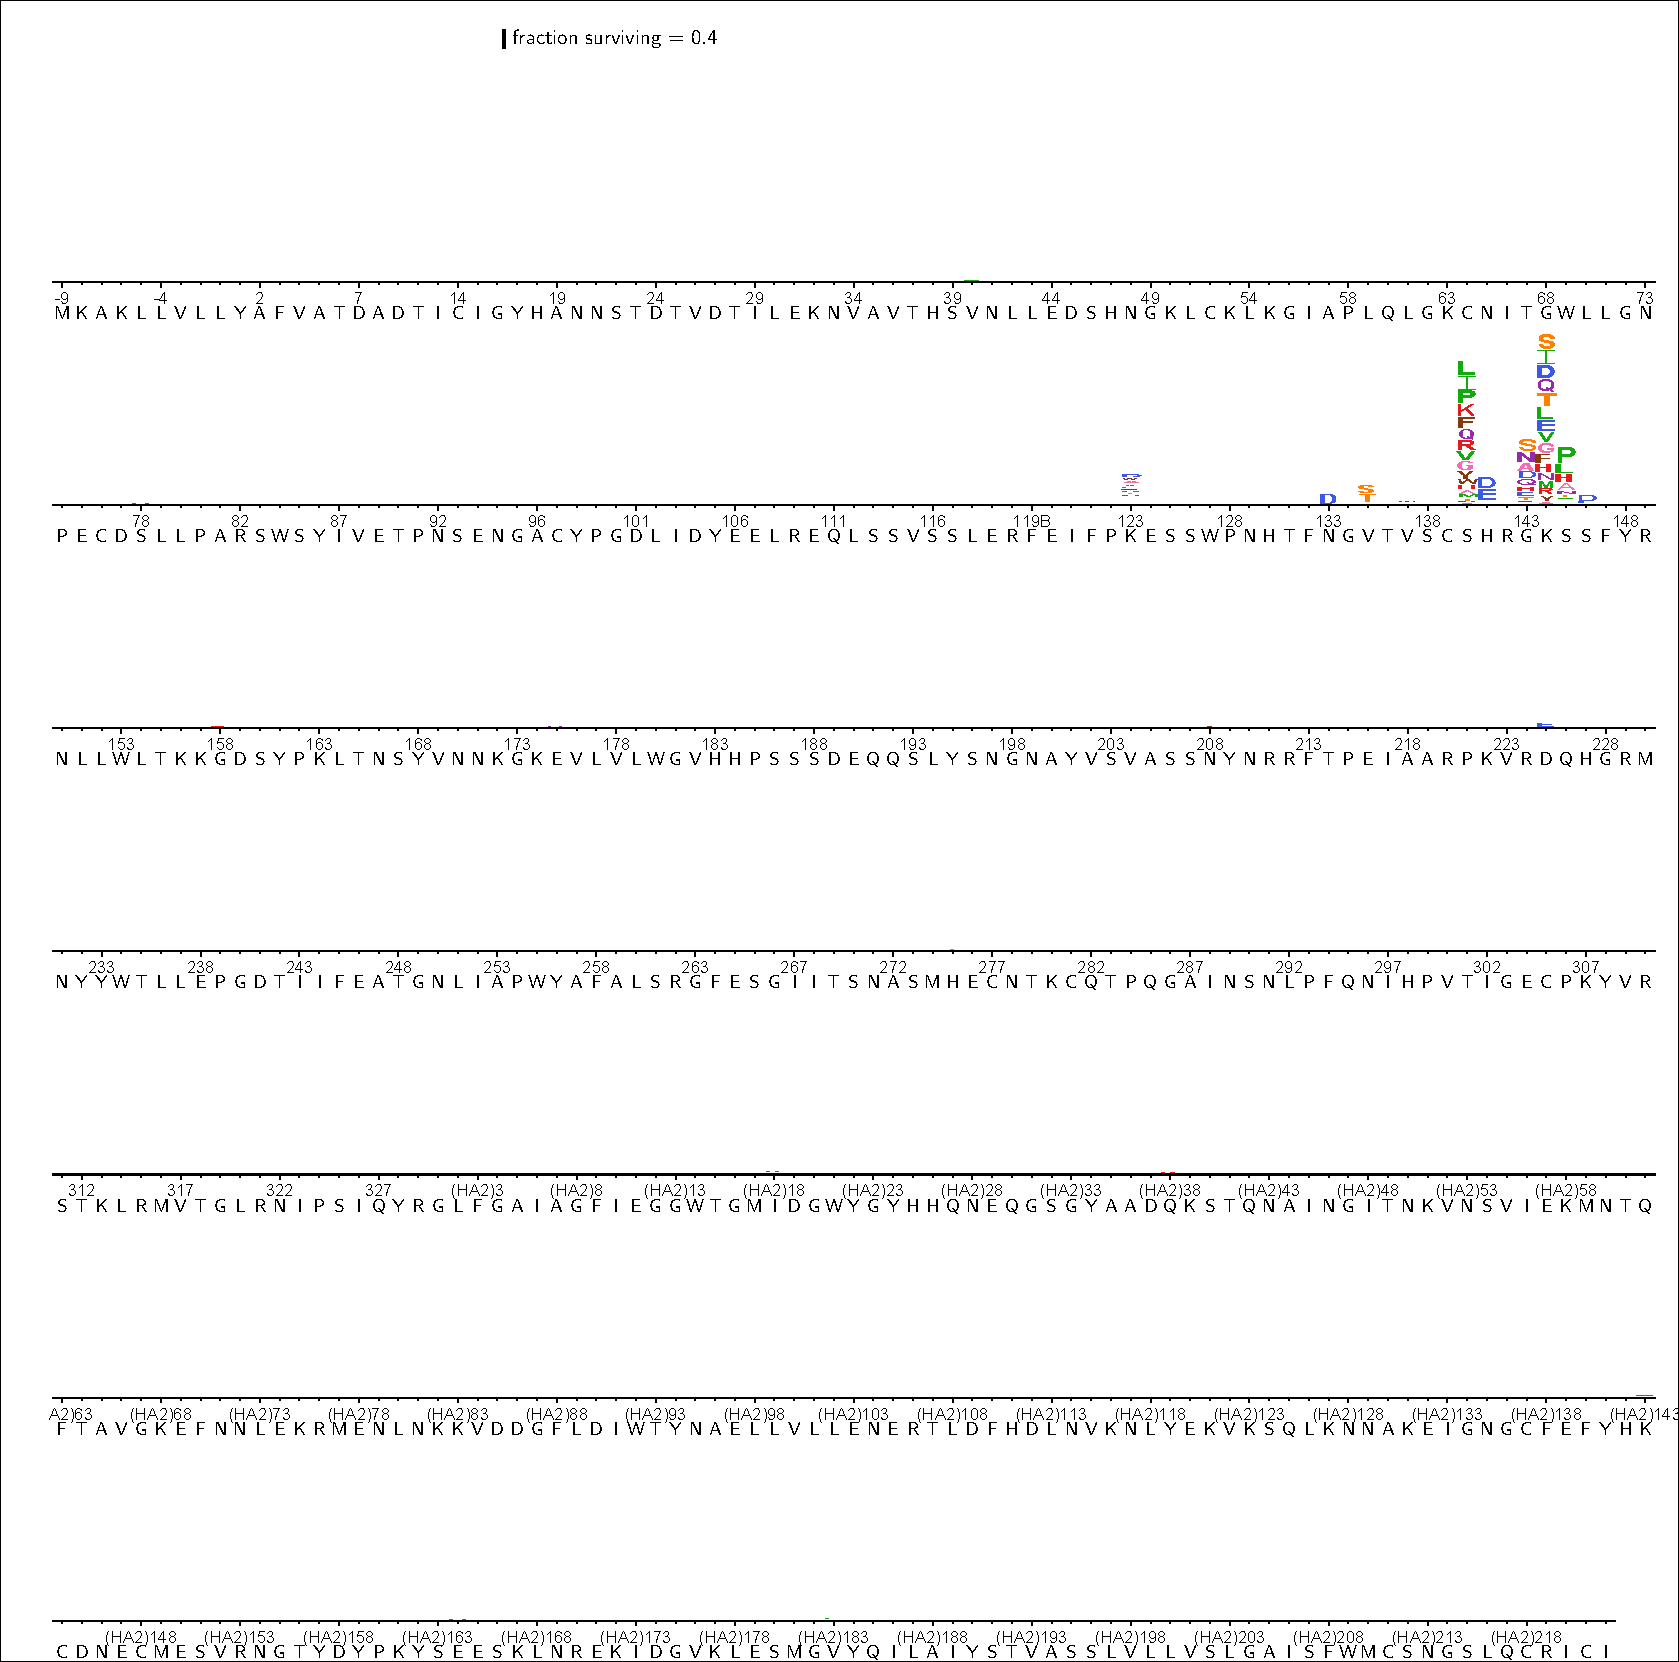
\includegraphics[trim=0.1cm 0.02cm 0.1cm 0.03cm,clip=true,width=\textwidth]{figs/logoplots/H17L19_fracsurvive.pdf}}
\caption{\label{suppfig:H17L19logo}
CAPTION}
\end{suppfigure}

\begin{suppfigure}
\centerline{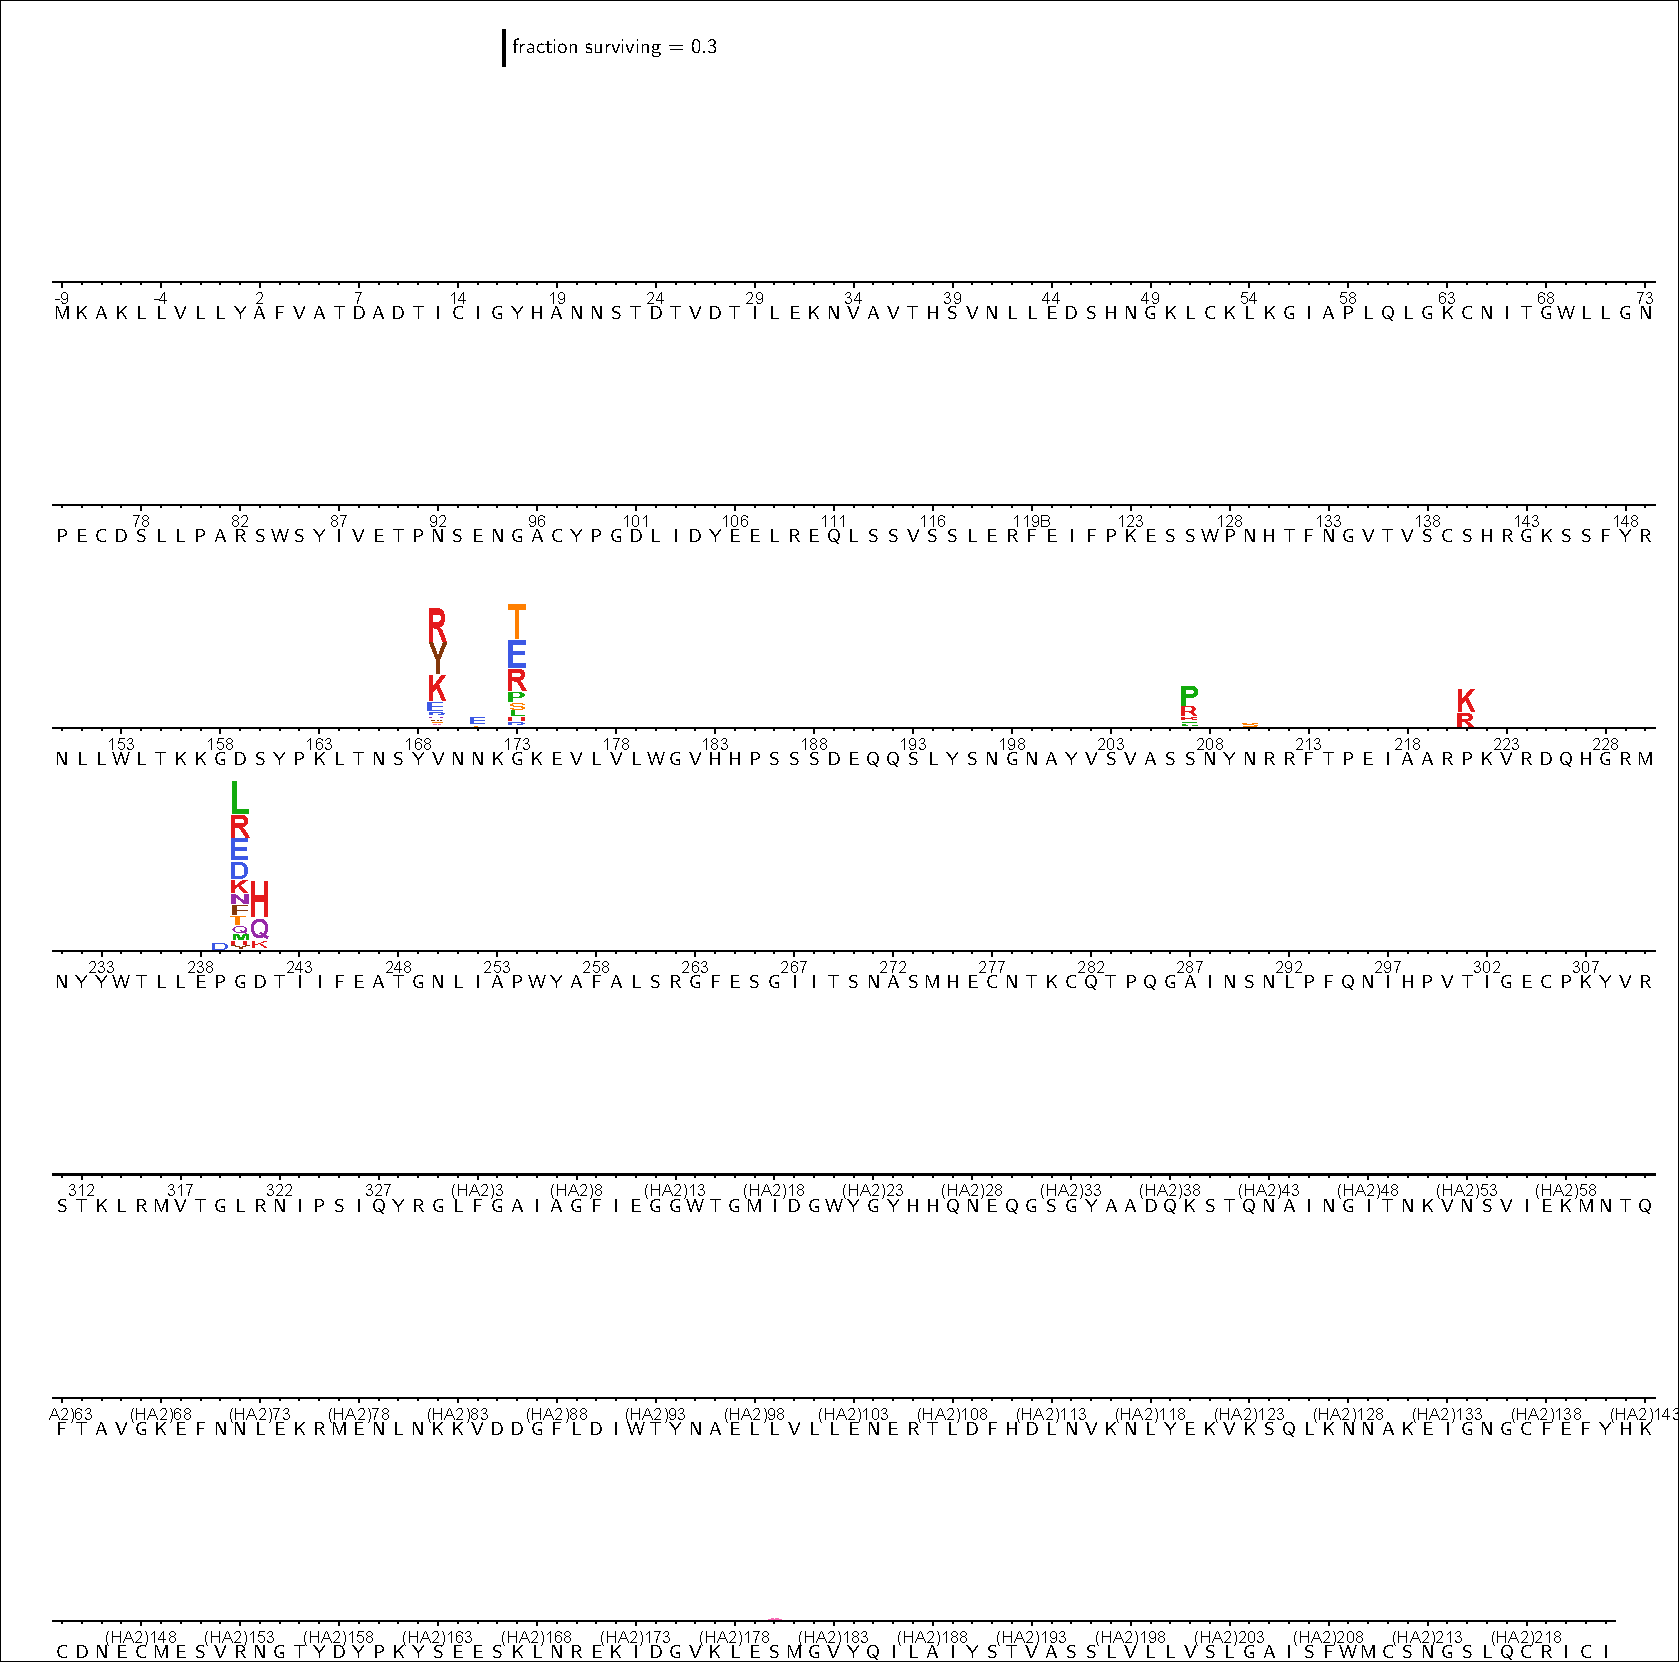
\includegraphics[trim=0.1cm 0.02cm 0.1cm 0.03cm,clip=true,width=\textwidth]{figs/logoplots/H17L10_fracsurvive.pdf}}
\caption{\label{suppfig:H17L10logo}
CAPTION}
\end{suppfigure}

\begin{suppfigure}
\centerline{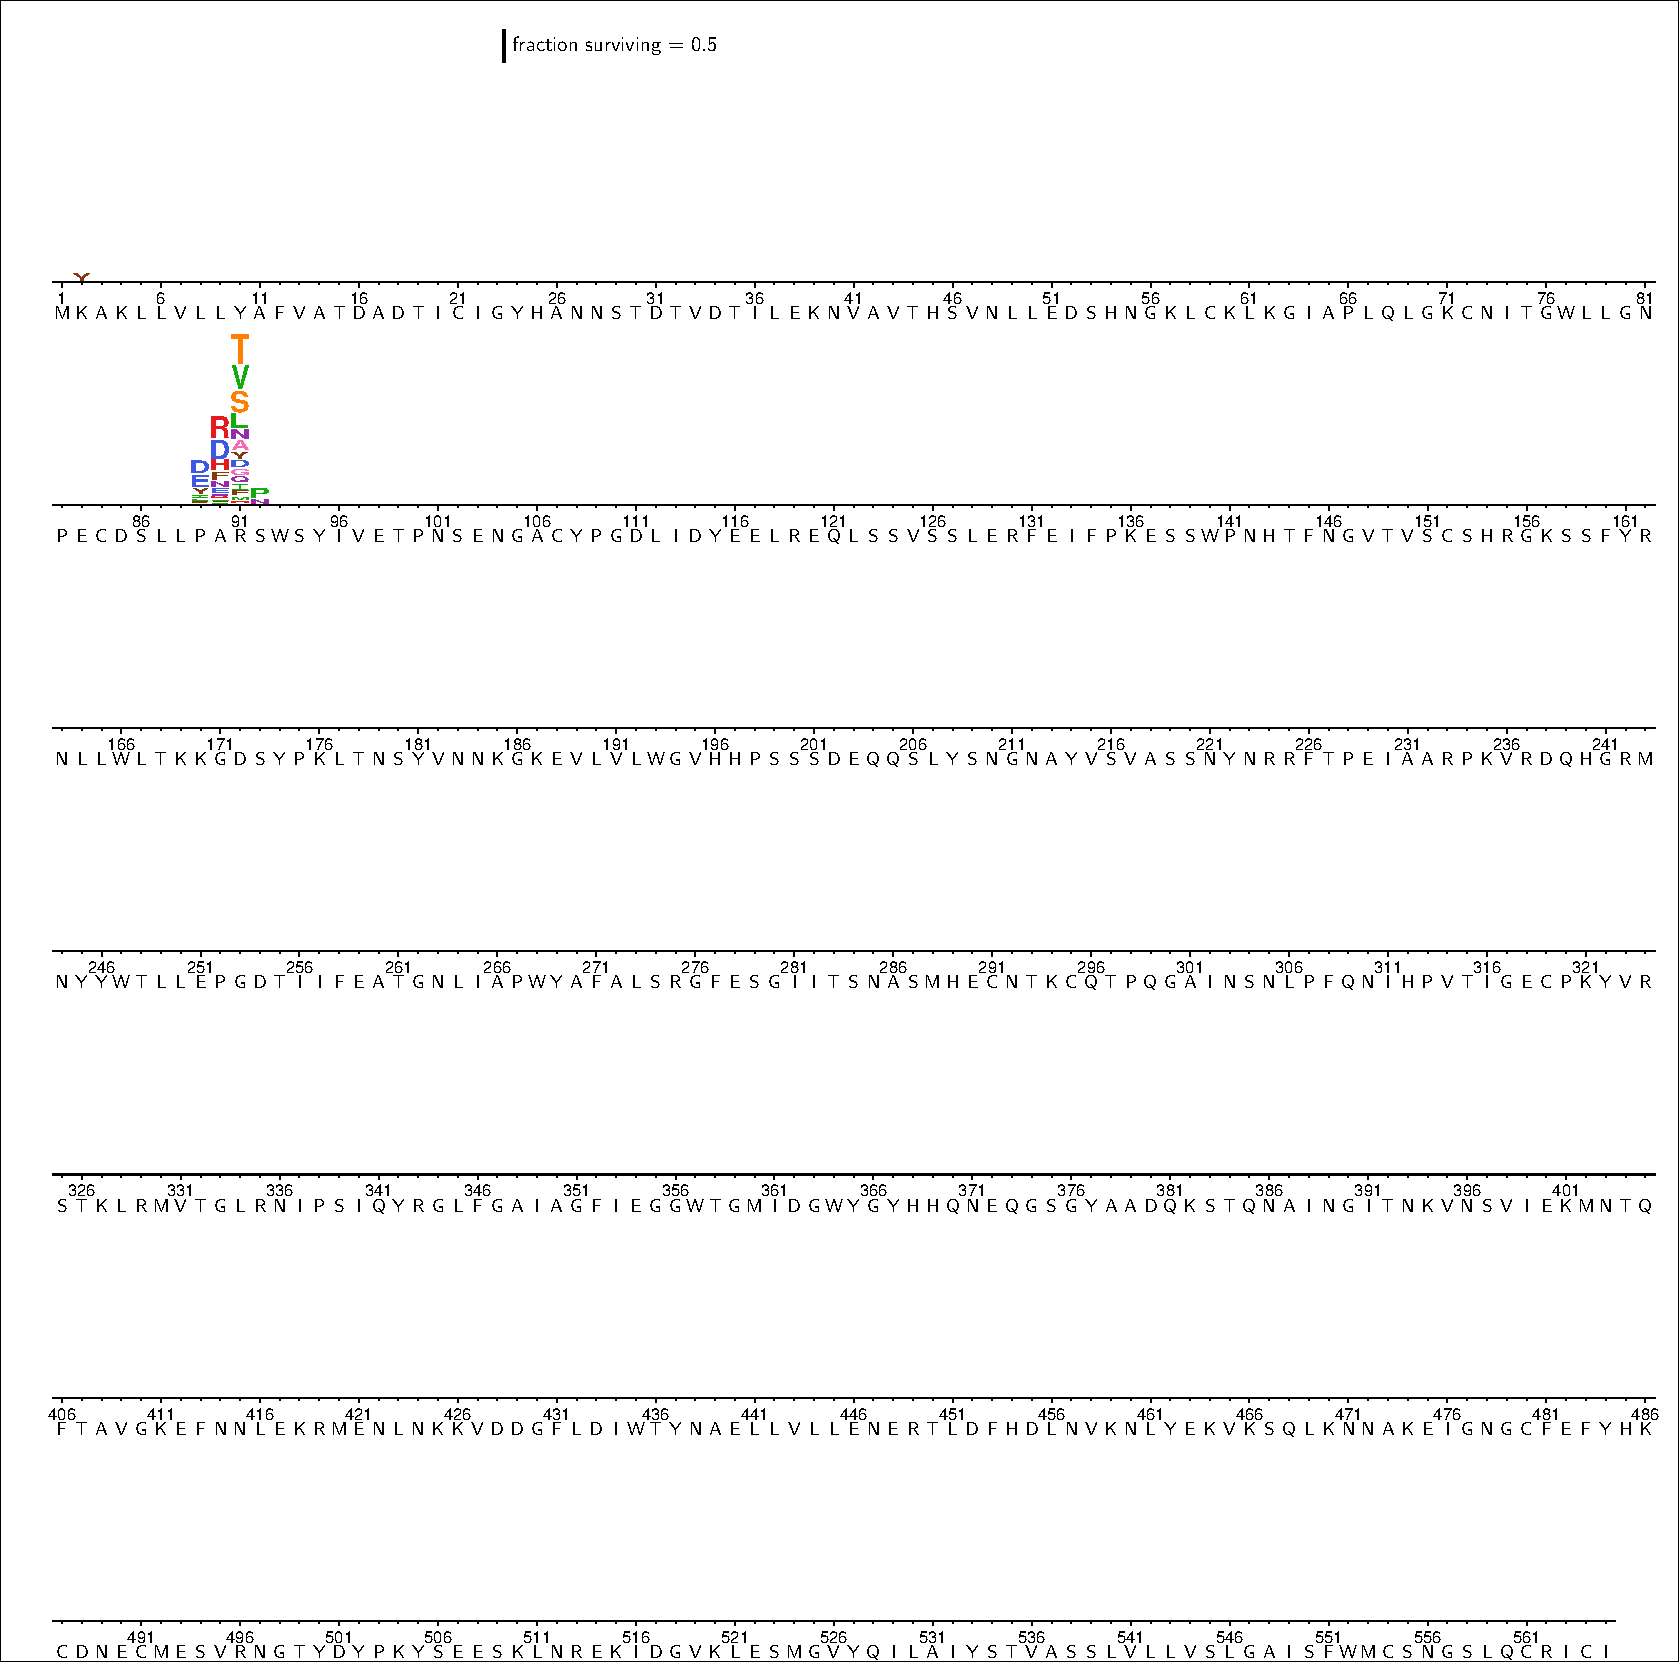
\includegraphics[trim=0.1cm 0.02cm 0.1cm 0.03cm,clip=true,width=\textwidth]{figs/logoplots/H17L7_fracsurvive.pdf}}
\caption{\label{suppfig:H17L7logo}
CAPTION}
\end{suppfigure}

\end{document}
